% ----------------- Documento ----------------- %
% Se define el tipo de documento (en este caso un artículo), en hoja A4 con tamaño de fuente de 11pt, escrito en castellano, e indicando que el documento tendrá páginas distintas a izquierda y derecha ("twoside"):
\documentclass[a4paper, 11pt, spanish, twoside]{article}
% Los demás tipos de documentos así como sus características y opciones pueden consultarse en: https://en.wikibooks.org/wiki/LaTeX/Document_Structure#Document_classes
% ---------------------------------------------- %


%%%%%%%%%%%%%%%%% - PREÁMBULO - %%%%%%%%%%%%%%%%% 

% ------------------ Página -------------------- %
% Se define el tamaño de las páginas, indicando el tamaño de los márgenes superior e inferior ("top" y "bottom"), e izquierdo y derecho ("left" y "right"):
\usepackage[top=2.5cm,bottom=2.5cm,left=2.5cm,right=2.5cm]{geometry}
% Se inserta el comando \raggedbottom para evitar que LaTeX rellene con espacios en blanco aquellas páginas que no alberguen suficiente contenido como para rellenarlas de forma "natural":
\raggedbottom 
% ---------------------------------------------- %


% ------------- Paquetes generales ------------- %
% Se importan distintos paquetes de propósito general:
\usepackage[utf8]{inputenc}
\usepackage[spanish]{babel}
\usepackage{float}
\usepackage{caption}
% ---------------------------------------------- %


% ------------ Paquetes específicos ------------ %
% Se importan distintos paquetes que será utilizados en momentos concretos del documento: 
\usepackage{pdfpages} % Para insertar la portada en formato PDF.
\usepackage{amssymb} % Para símbolos matemáticos.
\usepackage{bm} % Para negrita en símbolos matemáticos.
\usepackage{amsmath} % Para el entorno "split".
\usepackage[hidelinks]{hyperref} % Para urls.
\usepackage{longtable} % Para tablas largas.
\usepackage{graphicx} % Para insertar imágenes.
\usepackage{wrapfig} % Para posicionar imágenes alrededor del texto.
\usepackage{fontawesome5} % Para utilizar iconos de "fontawesome".
\usepackage{pdflscape}  % Para colocar páginas en formato apaisado.
\usepackage[T1]{fontenc}
\usepackage{textcomp}
\usepackage{lmodern} % Soluciona el problema de la mala resolución
\usepackage{url}

% ---------------------------------------------- %


% ---------------- Numeración ------------------ %
\counterwithin{table}{section} % Se numeran las tablas con respecto al capítulo en el que se encuentran.
\counterwithin{figure}{section} % Se numeran las figuras con respecto al capítulo en el que se encuentran.
\counterwithin{equation}{section} % Se numeran las ecuaciones con respecto al capítulo en el que se encuentran.
% ---------------------------------------------- %


% ------------- Página en blanco ----------------%
% Se define un comando (\blankpage) para insertar una página totalmente en blanco (sin número de página, encabezado y pie de página):
\usepackage{afterpage}
\newcommand\blankpage{%
    \null
    \thispagestyle{empty}%
    \newpage}
% ---------------------------------------------- %    


% ----------- Formato de los párrafos -----------%
% Se define el formato de los párrafos:
\setlength{\parindent}{0pt} % Se elimina la sangría en comienzo de párrafo (0pt).
\setlength{\parskip}{1em} % Se define el espacio entre dos párrafos (1em).
% ---------------------------------------------- %    

% -------------- Título adicional -------------- %
% Se añade una profundidad adicional a los títulos (profundidad 4):
\usepackage{titlesec}
\setcounter{secnumdepth}{4} % Se fija en 4 la profundidad de numeración de títulos.
\setcounter{tocdepth}{4} % Se fija en 4 la profundidad de títulos incluidos en el índice.
% Se modifica el formato de \paragraph (título de profundidad 4) para adaptarlo al formato del resto de títulos:
\titleformat{\paragraph}
{\normalfont\normalsize\bfseries}{\theparagraph}{1em}{}
\titlespacing*{\paragraph}
{0pt}{3.25ex plus 1ex minus .2ex}{1.5ex plus .2ex} 
% ---------------------------------------------- %    


% --------- Encabezado y pie de página -------- %
% El encabezado y pie de página forman parte del paquete fancyhdr:
\usepackage{fancyhdr}
\fancyhf{}
\pagestyle{fancy}

% Para solucionar error "headheight is too small":%
\setlength{\headheight}{14.6pt}
\addtolength{\topmargin}{-0.6pt}

% Se ajusta el tamaño de fuente para el encabezado y pie de página (9pt)
\fancyhf{\fontsize{2}{14}\selectfont}

% Contenido del encabezado (\fancyhead):
\fancyhead[RO]{Simulación de operación de una central nuclear} % Texto que se coloca en el encabezado de las páginas impares (O -> 'Odd', o impar) a la izquierda (R -> 'Odd')
\fancyhead[LE]{\nouppercase{\rightmark}} % Texto que se coloca en el encabezado de las páginas pares (E -> 'Even', o par) a la izquierda (L -> 'Left'). \rightmark se utiliza para insertar automáticamente el título de la sección correspondiente, y \nouppercase para que no aparezca todo en mayúsculas (formato por defecto de \rightmark).

% Contenido del pie de página (\fancyfoot):
\fancyfoot[RE]{Escuela  Técnica  Superior  de  Ingenieros  Industriales  (UPM)} % Texto que se coloca en el pie de página de las páginas pares (E -> 'Even', o par) a la derecha (R -> 'Right')
\fancyfoot[LO]{Antonio Dies Beneytez} % Texto que se coloca en el pie de página de las páginas impares (O -> 'Odd', o impar) a la izquierda (L -> 'Left')
\fancyfoot[LE,RO]{\thepage} % El número de página (\thepage) se coloca a la izquierda en las páginas pares y a la derecha en las impares.

% Se indica que sólo se quiere incorporar en \rightmark (utilizado más arriba) el título de la sección (y no de las subsecciones, subsubsecciones, etc.):
\renewcommand{\sectionmark}[1]{\markright{\thesection. #1}}
\renewcommand{\subsectionmark}[1]{}

% Formato de la línea de separación horizontal:
\renewcommand{\headrulewidth}{0.5pt} % Ancho de la línea del encabezado.
\renewcommand{\footrulewidth}{0.5pt} % Ancho de la línea del pie de página.
% ---------------------------------------------- % 


% ----------- Fragmentos de código ------------- %
% El paquete utilizado para insertar fragmentos de código en el documento es listings. En el presente bloque del preámbulo se definen ciertos parámetros de listings con el objetivo de adaptar dicho paquete a código escrito en Python.

\usepackage{listings} % Paquete para insertar código. 
\usepackage{xcolor} % Paquete para definir colores.

% Se definen los distintos colores que se utilizan para resaltar ciertos elementos del código:
\definecolor{codegreen}{rgb}{0.04314,0.6745,0.07843} % Verde.
\definecolor{codegray}{rgb}{0.5,0.5,0.5} % Gris.
\definecolor{codered}{rgb}{0.5373,0.02745,0.06275} % Rojo.
\definecolor{codeblue}{rgb}{0.071,0.0258,0.9882} % Azul.
\definecolor{codepurple}{rgb}{0.6,0.02745,0.5961} % Morado.

% Se define el color de fondo:
\definecolor{backcolour}{rgb}{0.95,0.95,0.92} % Gris oscuro.

% Se define el valor de ciertos parámetros de listings para adaptar dicho paquete a código escrito en Python:
\lstdefinestyle{mystyle}{
    % - General:
    language=Python, % Lenguaje de programación.
    basicstyle=\ttfamily\footnotesize, % Tipografía y tamaño de fuente.
    % - Colores de los distintos elementos del código:
    backgroundcolor=\color{backcolour}, % Color de fondo.  
    commentstyle=\color{codegray}, % Color de los comentarios.
    keywordstyle=\color{codeblue}, % Color de las palabras clave por defecto.
    stringstyle=\color{codegreen}, % Color de los "string"
    % - Palabras clave:
    deletekeywords={print}, % Se elimina "print" del conjunto de palabras clave para posteriormente asignarle el color morado.
    keywordstyle={[2]\ttfamily\color{codeblue}},
    keywords=[2]{as}, % Se añaden las palabras clave de color azul.
    keywordstyle={[3]\ttfamily\color{codepurple}},
    keywords=[3]{True, False, ttk, list, None, dict, zip, range, len, print, float, sum}, % Se añaden las palabras clave de color morado.
    keywordstyle={[4]\bfseries\ttfamily},
    keywords=[4]{_read_excel}, % Se añaden las palabras clave en negrita.
    emph={MyClass,__init__}, % Se añaden las palabras clave enfatizadas.   
    % - Números de línea:
    numberstyle=\tiny\color{codegray}, % Tamaño de fuente y color de los números de línea.
    numbers=left, % Se colocan los números de línea en el lado izquierdo.                 
    numbersep=5pt, % Separación horizontal de los números de línea.
    % - Saltos a la línea, espacios, indentación:
    breaklines=true, % Permitir saltos a la línea. 
    breakatwhitespace=true, % Saltar a la línea únicamente al encontrar espacios.
    postbreak = \mbox{{$\hookrightarrow$}\space}, % Se añade una flecha al cambiar de línea.
    showspaces=false, % No mostrar los espacios. 
    showstringspaces=false, % No mostrar los espacios en los "string".
    keepspaces=true, % Mantener los espacios presentes en el código. 
    tabsize=2, % Tamaño de indentación.
    % - Título:
    captionpos=b % Posición del título del fragmento de código (b=bottom - abajo).
} 
\lstset{style=mystyle} % Se asocia el estilo de listings al estilo que acaba de definirse ("mystyle")

% Se realizan una serie de operaciones complementarias con el paquete listings (su comprensión no es necesaria para manejar dicho paquete):
\makeatletter
\def\lst@OpLiteratekey#1\@nil@{\let\lst@ifxopliterate\lst@if
                             \def\lst@opliterate{#1}}
\lst@Key{opliterate}{}{\@ifstar{\lst@true \lst@OpLiteratekey}
                             {\lst@false\lst@OpLiteratekey}#1\@nil@}
\lst@AddToHook{SelectCharTable}
    {\ifx\lst@opliterate\@empty\else
         \expandafter\lst@OpLiterate\lst@opliterate{}\relax\z@
     \fi}
\def\lst@OpLiterate#1#2#3{%
    \ifx\relax#2\@empty\else
        \lst@CArgX #1\relax\lst@CDef
            {}
            {\let\lst@next\@empty
             \lst@ifxopliterate
                \lst@ifmode \let\lst@next\lst@CArgEmpty \fi
             \fi
             \ifx\lst@next\@empty
                 \ifx\lst@OutputBox\@gobble\else
                   \lst@XPrintToken \let\lst@scanmode\lst@scan@m
                   \lst@token{#2}\lst@length#3\relax
                   \lst@XPrintToken
                 \fi
                 \let\lst@next\lst@CArgEmptyGobble
             \fi
             \lst@next}%
            \@empty
        \expandafter\lst@OpLiterate
    \fi}

\lstset{ 
    literate={á}{{\'a}}1 {é}{{\'e}}1 {í}{{\'i}}1 {ó}{{\'o}}1 {ú}{{\'u}}1
  {Á}{{\'A}}1 {É}{{\'E}}1 {Í}{{\'I}}1 {Ó}{{\'O}}1 {Ú}{{\'U}}1
  {à}{{\`a}}1 {è}{{\`e}}1 {ì}{{\`i}}1 {ò}{{\`o}}1 {ù}{{\`u}}1
  {À}{{\`A}}1 {È}{{\'E}}1 {Ì}{{\`I}}1 {Ò}{{\`O}}1 {Ù}{{\`U}}1
  {ä}{{\"a}}1 {ë}{{\"e}}1 {ï}{{\"i}}1 {ö}{{\"o}}1 {ü}{{\"u}}1
  {Ä}{{\"A}}1 {Ë}{{\"E}}1 {Ï}{{\"I}}1 {Ö}{{\"O}}1 {Ü}{{\"U}}1
  {â}{{\^a}}1 {ê}{{\^e}}1 {î}{{\^i}}1 {ô}{{\^o}}1 {û}{{\^u}}1
  {Â}{{\^A}}1 {Ê}{{\^E}}1 {Î}{{\^I}}1 {Ô}{{\^O}}1 {Û}{{\^U}}1
  {Ã}{{\~A}}1 {ã}{{\~a}}1 {Õ}{{\~O}}1 {õ}{{\~o}}1
  {œ}{{\oe}}1 {Œ}{{\OE}}1 {æ}{{\ae}}1 {Æ}{{\AE}}1 {ß}{{\ss}}1
  {ű}{{\H{u}}}1 {Ű}{{\H{U}}}1 {ő}{{\H{o}}}1 {Ő}{{\H{O}}}1
  {ç}{{\c c}}1 {Ç}{{\c C}}1 {ø}{{\o}}1 {å}{{\r a}}1 {Å}{{\r A}}1
  {€}{{\euro}}1 {£}{{\pounds}}1 {«}{{\guillemotleft}}1
  {»}{{\guillemotright}}1 {ñ}{{\~n}}1 {Ñ}{{\~N}}1 {¿}{{?`}}1
  {º}{{\textordmasculine}}1}

\lstset{opliterate=
   *{0}{{{\color{codered}0}}}1 {1}{{{\color{codered}1}}}1 
   {2}{{{\color{codered}2}}}1 {3}{{{\color{codered}3}}}1 
   {4}{{{\color{codered}4}}}1 {5}{{{\color{codered}5}}}1 
   {6}{{{\color{codered}6}}}1 {7}{{{\color{codered}7}}}1 
   {8}{{{\color{codered}8}}}1 {9}{{{\color{codered}9}}}1}

\DeclareCaptionType{code}[Código][ÍNDICE DE CÓDIGOS] % Se define el entorno "Código" (de forma que al introducir un fragmento de código en el documento aparezca como: Código 1.1: ...), y la lista con los distintos códigos ("Índice de códigos").
\counterwithin{code}{section} % Se numeran los códigos con respecto al capítulo en el que se encuentran.
% ---------------------------------------------- % 


% --------------- Bibliografía ----------------- %
% El manejo de la bibliografía se realiza mediante el paquete biblatex:
\usepackage[backend=bibtex, style=authoryear, sorting=nyt, citestyle=authoryear, maxcitenames=2, maxbibnames=5, giveninits=true, uniquename=init]{biblatex} 

% Los distintos parámetros que aparecen en la línea anterior corresponden a las siguientes características de la bibliografía:
% - style: la manera en la que aparecen las referencias en la bibliografía. En este caso se opta por "authoryear", pero existen múltiples estilos posibles que se resumen en la siguiente guía: https://www.overleaf.com/learn/latex/biblatex_bibliography_styles.
% - sorting: orden en el que aparecen las distintas referencias en la bibliografía. En este caso se opta por ordenarlas en primer lugar por el apellido del primer autor, en segundo lugar por el año de publicación, y por último por el título de la publicación (nyt=name-year-title)
% - citestyle: elementos y orden de dichos elementos de una referencia al citarla en el documento. En este caso se escoge "authoryear" para que aparezca en primer lugar el apellido del autor (o de los autores) y en segundo lugar el año de publicación. Existe gran variedad de opciones en cuanto al parámetro citestyle que se resumen en: https://www.overleaf.com/learn/latex/biblatex_citation_styles.
% maxcitenames: máximo número de autores que aparecen al citar una referencia en el documento. Al escoger un valor de 2 para este parámetro se pueden dar los siguientes casos: un único autor -> (autor, año), dos autores -> (autor 1 y/e autor 2, año), tres o más autores -> (autor 1 et al., año).
% maxbibnames: parámetro idéntico al anterior pero para la bibliografía en lugar de las citas.
% giveinits y uniquename: para mostrar únicamente las iniciales de los nombres de los autores.

% Se importa el paquete csquotes para citar las referencias a lo largo del documento:
\usepackage{csquotes} 

% Se realizan una serie de operaciones para adaptar la bibliografía al estilo deseado (coma entre autor y año al citar una referencia, idioma castellano, etc.):
\DeclareNameAlias{sortname}{family-given}
\renewcommand*{\nameyeardelim}{\addcomma\space}
\setlength\bibitemsep{\baselineskip}
\DefineBibliographyStrings{spanish}{%
  andothers = {et\addabbrvspace al\adddot}
}

\makeatletter

\newrobustcmd*{\parentexttrack}[1]{%
  \begingroup
  \blx@blxinit
  \blx@setsfcodes
  \blx@bibopenparen#1\blx@bibcloseparen
  \endgroup}

\AtEveryCite{%
  \let\parentext=\parentexttrack%
  \let\bibopenparen=\bibopenbracket%
  \let\bibcloseparen=\bibclosebracket}

\makeatother

\addbibresource{content/sections/biblio.bib}

% --------------- Abreviaturas, unidades y acrónimos ----------------- %

\usepackage{glossaries}
\makenoidxglossaries

\newglossaryentry{simuladores}
{
    name=Simuladores,
    text={simuladores},
    description={Los simuladores son... Esto es un ejemplo para el glosario}
}

\newacronym{smr}{SMR}{Small Modular Reactors}
% ---------------------------------------------- % 

%%%%%%%%%%%% - INICIO DEL DOCUMENTO - %%%%%%%%%%%%

\begin{document} 

%%%%%%%%%%%%%%%%%%%%%%%%%%%%%%%%%%%%%%%%%%%%%%%%%%


%%%%%%%%%%%%%%%%%%% - PORTADA - %%%%%%%%%%%%%%%%%%

% Se comienza una página nueva sin formato (sin número de página y sin encabezado/pie de página), ya que sólo incorpora la la portada:
\newpage
\thispagestyle{empty}

% La portada se inserta mediante el comando \includepdf seguido del archivo PDF correspondiente (que se ajusta automáticamente a las dimensiones de la página):
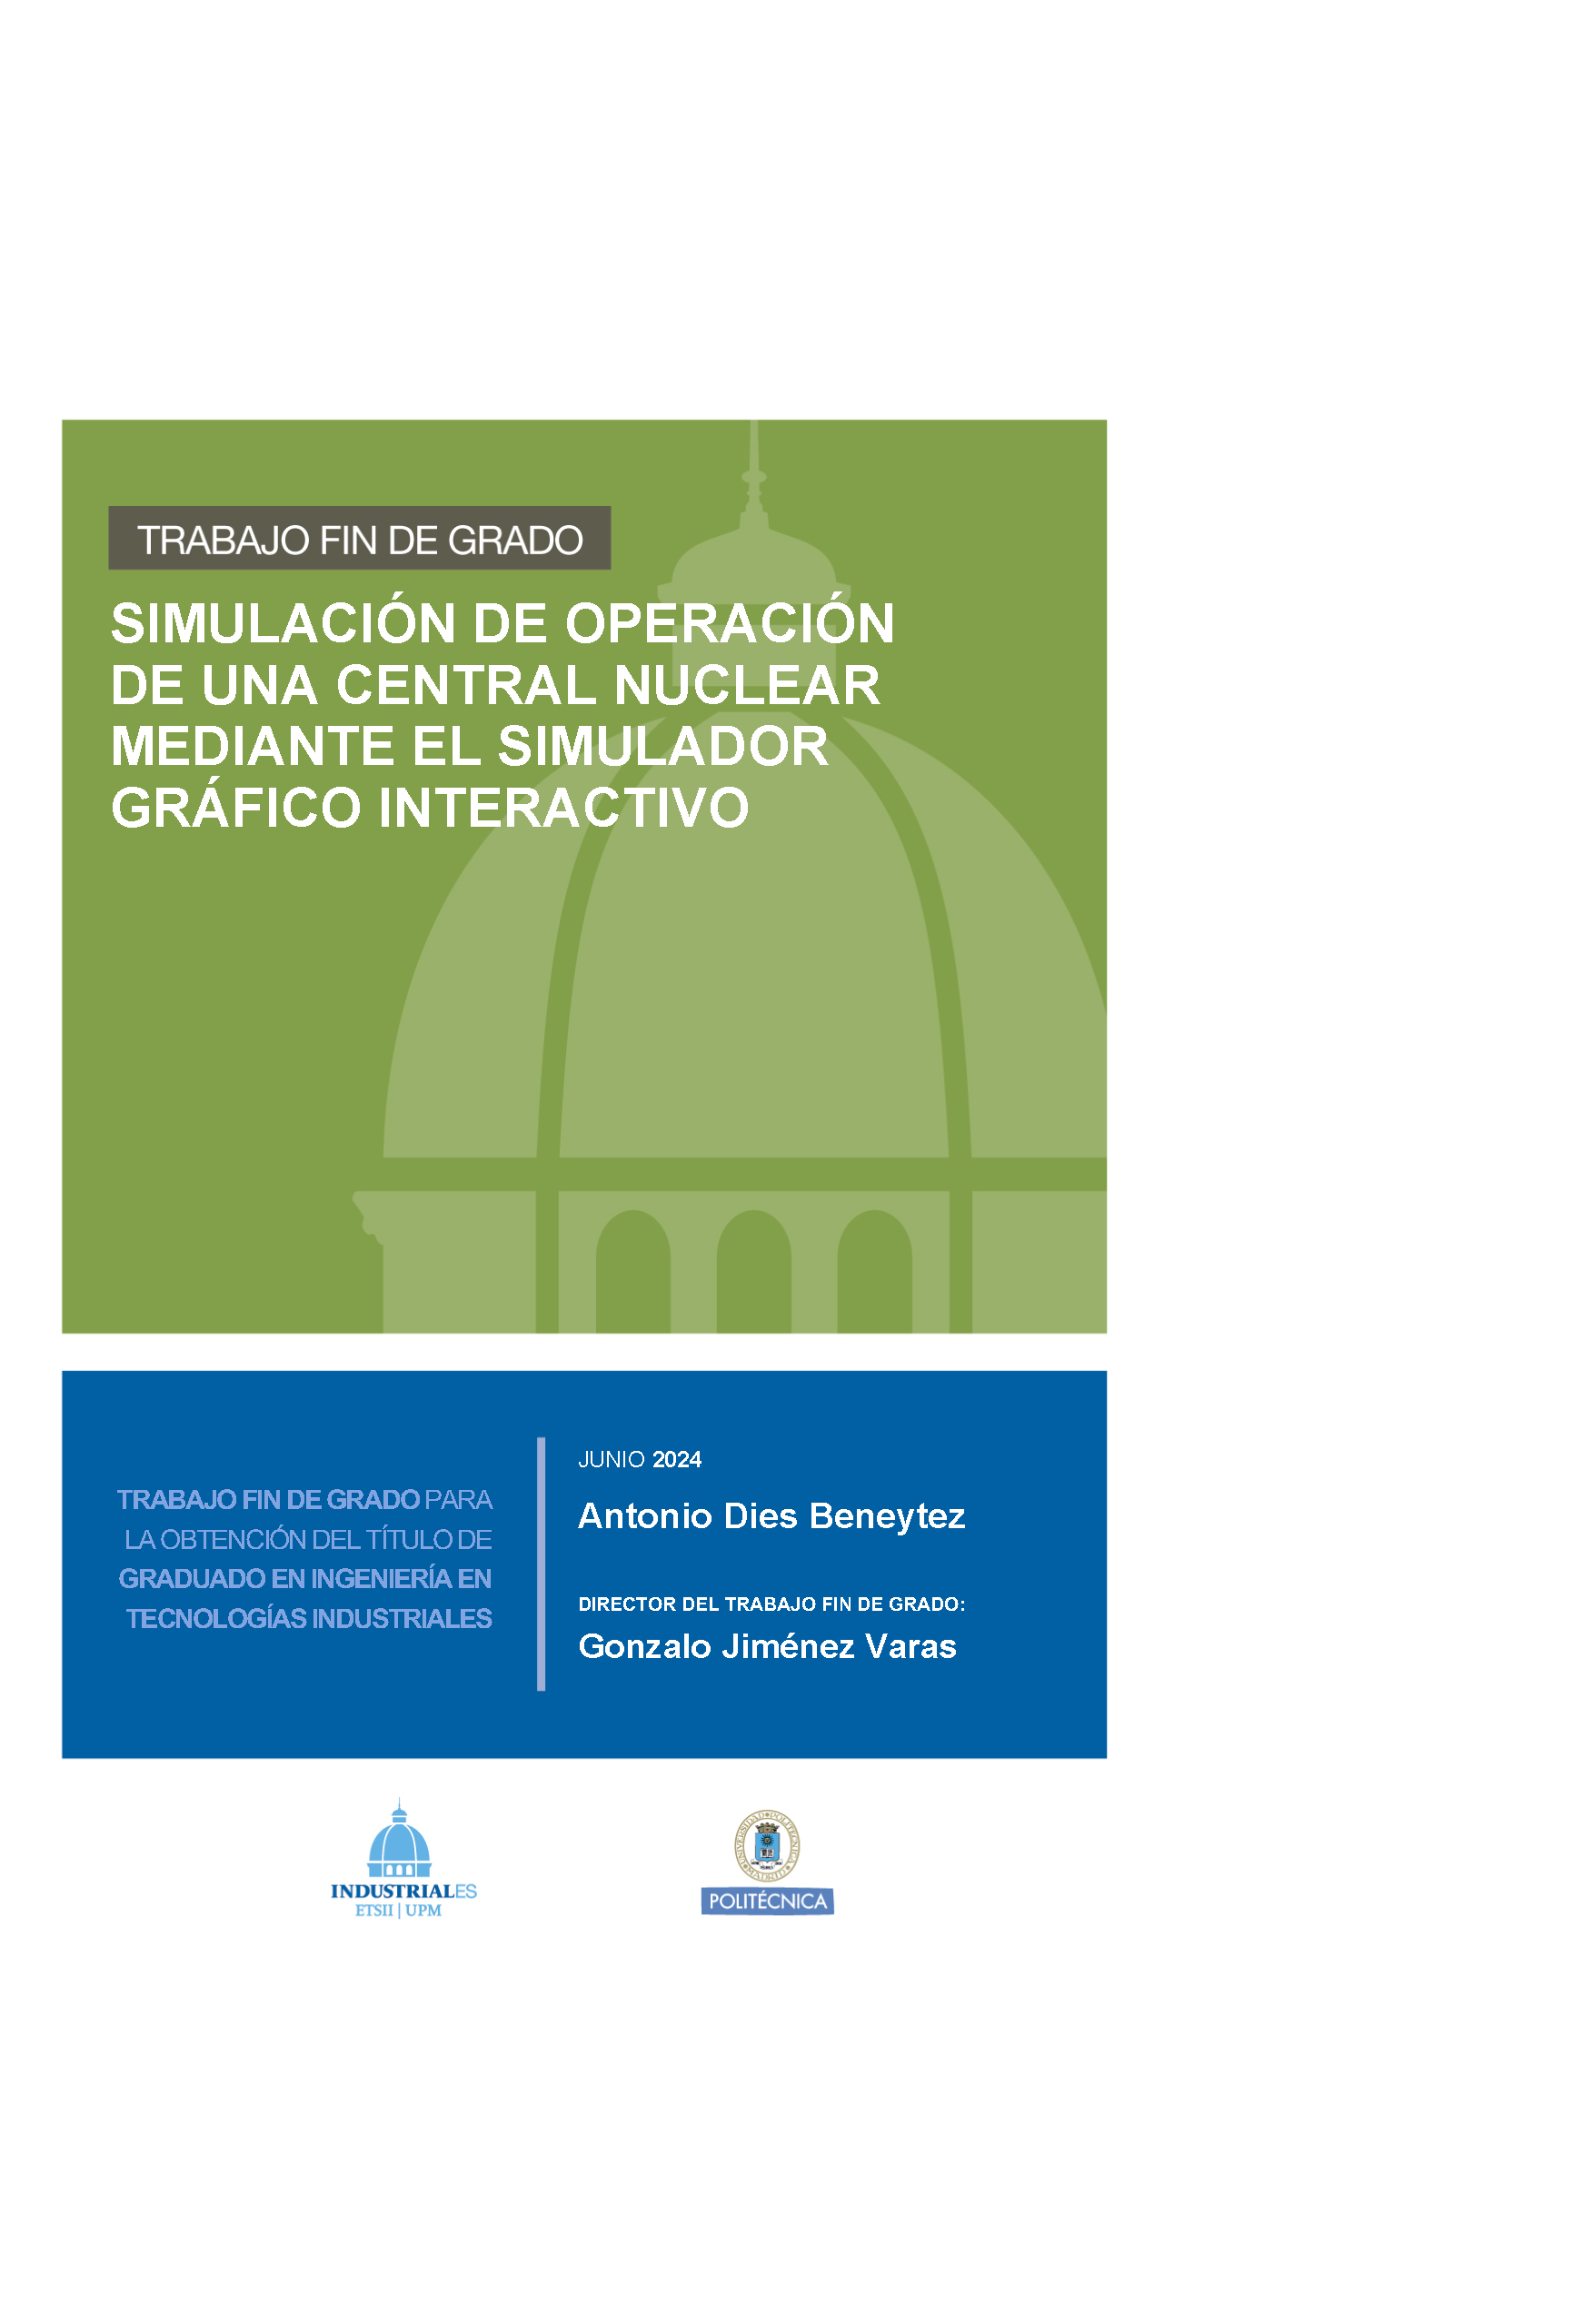
\includepdf{Portada_TFG_Antonio_Dies.pdf}

%%%%%%%%%%%%%%%%%%%%%%%%%%%%%%%%%%%%%%%%%%%%%%%%%%

% Las páginas anteriores al contenido del TFG/TFM (previas a la introducción) suelen numerarse de forma distinta a las del cuerpo del informe, en este caso en números romanos:
\pagenumbering{roman}

%%%%%%%%%%%%%%%%%%%%%%%%%%%%%%%%%%%%%%%%%%%%%%%%%%


%%%%%%%%%%%%%$%%%%% - CITA - %%%%%%%%%%%%%%%%%%%%%
 
% Se comienza una página nueva sin formato (sin número de página y sin encabezado/pie de página), ya que sólo incorpora la cita:
\newpage
\thispagestyle{empty}

\begin{flushright} % Se alinea el texto en el lado derecho de la página.
\vspace*{5cm} % Se añade un espacio vertical de 5cm para situar la cita en ~1/3 de la página.

\textit{“La cita del trabajo iría aquí”} 

\medskip % Salto a la línea de tamaño medio (existen \smallskip, \medskip y \bigskip)
- El autor de la cita 

\end{flushright}

\afterpage{\blankpage} % Se añade una página en blanco después de la cita.

%%%%%%%%%%%%%%%%%%%%%%%%%%%%%%%%%%%%%%%%%%%%%%%%%%


%%%%%%%%%%%%% - AGRADECIMIENTOS - %%%%%%%%%%%%%%%%

% Se comienza una página nueva con formato plano (sin encabezado/pie de página pero con número de página):
\newpage
\thispagestyle{plain}

\section*{AGRADECIMIENTOS} % Se añade un asterisco a \section para que el título no esté numerado.
\addcontentsline{toc}{section}{AGRADECIMIENTOS} % Al utilizar \section* se ha de añadir manualmente el apartado al índice (Table Of Contents, TOC).

Agradezco a \dots

Gracias a \dots

A \dots \ por \dots

\afterpage{\blankpage} % Se añade una página en blanco después de los agradecimientos.

%%%%%%%%%%%%%%%%%%%%%%%%%%%%%%%%%%%%%%%%%%%%%%%%%%


%%%%%%%%%%%%%% - RESUMEN EJECUTIVO - %%%%%%%%%%%%%

\newpage
\section*{RESUMEN} % Se añade un asterisco a \section para que el título no esté numerado.
\markright{RESUMEN} % Al utilizar \section* se ha de añadir manualmente el título del apartado al encabezado.
\addcontentsline{toc}{section}{RESUMEN} % Al utilizar \section* se ha de añadir manualmente el apartado al índice (Table Of Contents, TOC).

Este documento constituye una guía (que sirve a su vez de plantilla) para la elaboración de informes de TFG o TFM en \LaTeX. No pretende abarcar todas y cada una de las funcionalidades que ofrece \LaTeX \ (¡las posibilidades son prácticamente infinitas!) pero sí tratar los aspectos fundamentales para la elaboración de un documento utilizando esta indispensable herramienta. Además de los elementos básicos de cualquier informe (índice, tablas, ecuaciones, bibliografía, etc.), esta guía incluye ``tutoriales'' y plantillas para algunos de los elementos presentes en todo (o casi todo) informe de TFG o TFM (como son el diagrama de Gantt o la EDP). 

\textbf{Nota:} se ha tratado de explicar con detalle la mayor parte de elementos presentes en el documento, ya sea por medio de los capítulos y apartados que lo conforman o mediante explicaciones bajo la forma de comentarios en el código \LaTeX. Es especialmente importante examinar con atención el preámbulo de dicho código, ya que en él se llevan a cabo muchas de las operaciones esenciales que dan forma al documento.

\afterpage{\blankpage} % Se añade una página en blanco después del resumen.

%%%%%%%%%%%%%%%%%%%%%%%%%%%%%%%%%%%%%%%%%%%%%%%%%%


%%%%%%%%%%%%%%%%%%% - ÍNDICE - %%%%%%%%%%%%%%%%%%%

\newpage

\renewcommand*\contentsname{ÍNDICE} % Se modifica el nombre por defecto de la "Table Of Contents" (tabla de contenidos, índice) para pasar a llamarla "ÍNDICE".

\tableofcontents % Se genera el índice de contenidos del documento que incorpora todos los títulos de \section, \subsection y \subsubsection (y también \paragraph, ver capítulo 1), así como los títulos añadidos con \addcontentsline (como el resumen ejecutivo, por ejemplo).

\afterpage{\blankpage} % Se añade una página en blanco después del índice.


%%%%%%%%%%%%%%%%%%%%%%%%%%%%%%%%%%%%%%%%%%%%%%%%%%

% Se inicia una nueva página, y se restablece la numeración de las páginas, utilizando esta vez el sistema de numeración estándar (1, 2, 3, 4, ...)
\newpage
\pagenumbering{arabic}

%%%%%%%%%%%%%%%%%%%%%%%%%%%%%%%%%%%%%%%%%%%%%%%%%%


%%%%%%%%%%%%%%%%%%% - TÍTULOS - %%%%%%%%%%%%%%%%%%

\section{TÍTULOS} \label{sec:titulos}

En los documentos de clase \texttt{article} (los distintos tipos de documentos disponibles así como sus diferentes aplicaciones pueden consultarse en \url{https://en.wikibooks.org/wiki/LaTeX/Document_Structure#Document_classes}) existen por defecto tres profundidades de títulos numerados, en orden jerárquico: \texttt{\textbackslash section}, \texttt{\textbackslash subsection} y \texttt{\textbackslash subsubsection}. El título del presente capítulo es un ejemplo de título de profundidad 1 (comando \texttt{\textbackslash section}).


\subsection{Profundidad 2}

Hola que tal. Este es un ejemplo de título de profundidad 2 (comando \texttt{\textbackslash subsection}) que, como se puede ver, queda automáticamente numerado con respecto al título jerárquicamente superior (profundidad 1) inmediatamente anterior.


\subsubsection{Profundidad 3}

Este es un ejemplo de título de profundidad 3 (comando \texttt{\textbackslash subsubsection}) que, de nuevo, se numera automáticamente con respecto al título jerárquicamente superior (profundidad 2) inmediatamente anterior.


\paragraph{Profundidad 4}

En este documento se añade una profundidad de títulos numerados adicional (mediante los comandos \texttt{\textbackslash setcounter\{secnumdepth\}\{4\}} y \texttt{\textbackslash setcounter\{tocdepth\}\{4\}}, ver preámbulo para más información). Así, el comando \texttt{\textbackslash paragraph} se utiliza para incorporar títulos de profundidad 4, como en el caso del título del presente apartado. 

Si se quisiera aumentar en un grado más la profundidad de títulos, bastaría con asignar el valor 5 a ambos comandos \texttt{\textbackslash setcounter} (\texttt{\textbackslash setcounter\{secnumdepth\}\{5\}} y \texttt{\textbackslash setcounter\{tocdepth\} \{5\}}), y realizar los cambios pertinentes en el comando \texttt{\textbackslash subparagraph} de modo que su formato sea coherente con el del resto de títulos (de la misma forma que lo realizado con el comando \texttt{\textbackslash paragraph}, ver preámbulo para más información)


\subsection{Formato y numeración}

La numeración así como el formato de los títulos (tamaño de fuente, tipografía, etc.) utilizados en este documento corresponden a los valores por defecto (excepto en el caso de \texttt{\textbackslash paragraph}, como se explica más arriba), pero pueden ser modificados en el preámbulo del documento (una breve guía sobre la personalización del formato de los títulos puede consultarse en \url{https://www.overleaf.com/learn/latex/sections_and_chapters#Customize_chapters_and_sections}). 

En caso de que no se quiera numerar alguno de los títulos, basta con añadir un asterísco (\textbf{*}) al comando correspondiente, como por ejemplo \texttt{\textbackslash subsection*\{Título sin numerar\}}:


\subsection*{Título sin numerar} 
\addcontentsline{toc}{subsection}{Título sin numerar}

Los títulos sin numerar no aparecen en la tabla de contenidos (índice), pero pueden ser añadidos con ayuda del comando \texttt{\textbackslash addcontentsline\{toc\}} (utilizado previamente para los apartados de Agradecimientos y Resumen ejecutivo), que en este caso quedaría como: \texttt{\textbackslash addcontentsline\{toc\} \ \{subsection\}\{Título sin numerar\}}.


\subsection{Referencias con el comando \texttt{\textbackslash label}} \label{sec:referencias}

Los comandos \texttt{\textbackslash label} se utilizan en \LaTeX \ para colocar referencias que puedan ser utilizadas a lo largo del documento. Son especialmente útiles, como se verá más adelante, para referirse a elementos del documento como tablas, imágenes, diagramas, etc., pero también pueden ser utilizados para referirse a capítulos o secciones del informe. 

Para citar una referencia basta con utilizar el comando \texttt{\textbackslash ref} en el interior del cual se indica aquello a lo que se quiere hacer referencia, como por ejemplo al primer capítulo de este documento, el capítulo \ref{sec:titulos}.

\textbf{Nota:} ya que el comando \texttt{\textbackslash label} es compartido por títulos, figuras, tablas, etc., es bastante útil utilizar una nomenclatura clara para definir cada referencia, por ejemplo: ``tab:" \ seguido del nombre de la tabla para las tablas, ``fig:" \ seguido del nombre de la figura para las figuras, etc.

%%%%%%%%%%%%%%%%%%%%%%%%%%%%%%%%%%%%%%%%%%%%%%%%%%


%%%%%%%%%%%%%% - FORMATO DE TEXTO - %%%%%%%%%%%%%%

\newpage
\section{FORMATO DE TEXTO} \label{sec:formato}

Como en cualquier editor de texto, el formato del texto puede alterarse sobre la marcha de distintas maneras. Pueden incluirse palabras en \textbf{negrita} (si se utiliza Overleaf puede utilizarse el atajo \texttt{ctrl+B} en Windows o \texttt{Cmd+B} en Mac), palabras en \textit{curiva} (\texttt{ctrl+I} o \texttt{Cmd+I}), o una \textit{\textbf{combinación}} de ambas.


\subsection{Tamaño de fuente}

También se puede modificar el {\huge tamaño} de forma {\footnotesize rápida} y {\Large sencilla} (una lista con los distintos tamaños y sus comandos respectivos puede encontrarse en \url{https://www.sascha-frank.com/latex-font-size.html})


\subsection{Color}

\definecolor{coral}{rgb}{1.0, 0.5, 0.31}

El \textcolor{teal}{color} del \textcolor{purple}{texto} también puede ser modificado sobre la marcha, así como subrayar ciertas \colorbox{lightgray}{palabras} o \colorbox{yellow}{bloques de palabras}. Algunos colores están implementados por defecto y pueden utilizarse indicando simplemente su denominación (red, orange, blue, etc., resumidos en esta \href{https://i.stack.imgur.com/tmoHS.png}{\textcolor{blue}{imagen}}), pero también pueden definirse colores mediante sus códigos rgb, RGB, HTML, o cmyk, haciendo uso del paquete \texttt{xcolor}. Por ejemplo: \textbackslash \texttt{definecolor\{coral\}\{rgb\}\{1.0, 0.5, 0.31\}\definecolor{coral}{rgb}{1.0, 0.5, 0.31}} define un color con el correspondiente identificador rgb que se puede utilizar de ahora en adelante haciendo uso del nombre que se le ha asignado, \textcolor{coral}{coral} (una extensa guía con gran variedad de colores puede consultarse en \url{http://latexcolor.com/})


\subsection{Espaciado}

Puede ser de utilidad insertar \hspace{0.5cm} espacios \hspace{1cm} entre distintas \hspace{2cm} palabras, o espacios verticales entre párrafos u otros elementos del documento,

\vspace{6cm}

como en este caso.

Aunque \textbackslash\texttt{hspace} y \textbackslash\texttt{vspace} presenten la ventaja de ser totalmente personalizables, para espaciados de tamaño estándar es recomendable utilizar \textbackslash \ (espacio) y \textbackslash\textbackslash \ (salto de línea).


\subsection{Listas}

Existen dos tipos de listas, las numeradas y las no numeradas.


\subsubsection{Listas no numeradas}

Las listas no numeradas corresponden al entorno \texttt{itemize}:

\begin{itemize}
    \item Primer elemento.
    \item Segundo elemento.
\end{itemize}

Se pueden hacer listas de distintos niveles de profundidad:

\begin{itemize}
    \item Primer elemento.
    \item Segundo elemento.
    \begin{itemize}
        \item Tercer elemento.
        \begin{itemize}
            \item Cuarto elemento.
            \item Quinto elemento.
        \item Sexto elemento.
        \end{itemize}
        \item Séptimo elemento.
        \begin{itemize}
            \item Octavo elemento.
        \end{itemize}
    \end{itemize}
    \item Noveno elemento.
\end{itemize}


\subsubsection{Listas numeradas}

Las listas numeradas corresponden al entorno \texttt{enumerate}:

\begin{enumerate}
    \item Primer elemento
    \item Segundo elemento
    \item Tercer elemento
\end{enumerate}

Del mismo modo, las listas numeradas pueden incorporar distintos niveles de profundidad:

\begin{enumerate}
    \item Primer elemento
    \begin{enumerate}
        \item Segundo elemento
        \item Tercer elemento
        \begin{enumerate}
            \item Cuarto elemento
            \begin{enumerate}
                \item Quinto elemento
                \item Sexto elemento
            \end{enumerate}
            \item Séptimo elemento
        \end{enumerate}
        \item Octavo elemento
        \item Noveno elemento
    \end{enumerate}
    \item Décimo elemento.
\end{enumerate}


\subsubsection{Listas combinadas}

Las listas numeradas y no numeradas pueden combinarse, por ejemplo:

\begin{itemize}
    \item Primer elemento.
    \begin{enumerate}
        \item Segundo elemento
        \item Tercer elemento
        \begin{itemize}
            \item Cuarto elemento
            \item Quinto elemento
            \begin{enumerate}
                \item Sexto elemento
                \item Séptimo elemento
            \end{enumerate}
            \item Octavo elemento
        \end{itemize}
        \item Noveno elemento
    \end{enumerate}
    \item Décimo elemento
\end{itemize}


\subsubsection{Formato de las listas}

Tanto el estilo de las distintas numeraciones dentro de una lista numerada como la apariencia de los \textit{bullet points} de las listas no numeradas pueden personalizarse:

\renewcommand{\labelenumi}{\Roman{enumi}} % Primera profundidad de la lista numerada: números romanos (\Roman)
\renewcommand{\labelenumii}{\Alph{enumii}} % Segunda profundidad de la lista numerada: letras en mayúsculas (\Alph)
\renewcommand{\labelitemi}{\textbullet} % Primera profundidad de la lista no numerada: puntos (\textbullet).
\renewcommand{\labelitemii}{\textasteriskcentered} % Segunda profundidad de la lista no numerada: asteriscos (\textasteriskcentered) 

\begin{itemize}
    \item Primer elemento.
    \begin{enumerate}
        \item Segundo elemento
        \item Tercer elemento
        \begin{itemize}
            \item Cuarto elemento
            \item Quinto elemento
            \begin{enumerate}
                \item Sexto elemento
                \item Séptimo elemento
            \end{enumerate}
            \item Octavo elemento
        \end{itemize}
        \item Noveno elemento
    \end{enumerate}
    \item Décimo elemento
\end{itemize}

Los distintos formatos posibles pueden consultarse en la guía elaborada por Overleaf que puede encontrarse en \url{https://www.overleaf.com/learn/latex/lists}.

%%%%%%%%%%%%%%%%%%%%%%%%%%%%%%%%%%%%%%%%%%%%%%%%%%


%%%%%%%%%%%%%%%%%%% - TABLAS - %%%%%%%%%%%%%%%%%%%

\newpage
\section{TABLAS} \label{sec:tablas}

Las tablas se definen en el entorno \texttt{table}. Existen infinidad de posibilidades en cuanto a su formato: omitir o dibujar líneas horizontales y verticales, fusionar columnas y filas, alinear el contenido a la derecha, izquierda o centro, y demás opciones resumidas en \url{https://www.overleaf.com/learn/latex/tables}. Dado que la forma de construir una tabla directamente en código \LaTeX \ está lejos de ser cómoda e intuitiva, quizás lo más recomendable sea acudir a editores de tablas que generan automáticamente el código correspondiente y cuya interfaz es similar a la que puede encontrarse en Excel, como por ejemplo \url{https://www.tablesgenerator.com/}. Un ejemplo sencillo de tabla se muestra a continuación:

\vspace{25pt}

\begin{table}[H]
\centering
\begin{tabular}{|c|c|c|l|}
\hline
$\bm{n}$ & $\bm{a_n}$ & $\bm{a_{n+1}}$ & $\bm{\varphi} \ _{(= a_{n+1}/a_n)}$ \\ \hline\hline
\textbf{1} & 1 & 1 & 1 \\ \hline
\textbf{2} & 1 & 2 & 2 \\ \hline
\textbf{3} & 2 & 3 & 1,5 \\ \hline
\textbf{4} & 3 & 5 & 1,66666667 \\ \hline
\textbf{5} & 5 & 8 & 1,6 \\ \hline
\textbf{6} & 8 & 13 & 1,625 \\ \hline
\textbf{7} & 13 & 21 & 1,61538462 \\ \hline
\textbf{8} & 21 & 34 & 1,61904762 \\ \hline
\textbf{9} & 34 & 55 & 1,61764706 \\ \hline
\textbf{10} & 55 & - & - \\ \hline
\end{tabular}
\caption{Cinco primeros términos de la sucesión de Fibonacci}
\label{tabla:fibonacci5}
\end{table}

\vspace{5pt}

El título de la tabla se indica mediante el comando \textbackslash\texttt{caption} (este comando no solamente sirve para añadir un título a la tabla, sino que es esencial para que ésta aparezca en el índice de tablas), y, al igual que en el caso de los títulos de capítulos (ver apartado \ref{sec:referencias}), es muy recomendable añadir el comando \textbackslash\texttt{label} para poder referirse a la tabla en cuestión en partes posteriores (o anteriores) del documento.


\subsection{Posicionamiento}

Las tablas (al igual que otros elementos como imágenes o diagramas, como se verá más adelante) pueden posicionarse en distintos lugares de la página y en distintas posiciones con respecto al texto. La forma más común de situar una tabla es inmediatamente después de un párrafo y centrada en la página (como en el caso de la tabla \ref{tabla:fibonacci5}), lo que se consigue indicando \texttt{[H]} al iniciar el entorno \texttt{table} y añadiendo el comando \textbackslash\texttt{centering}, respectivamente. Una guía que recopila las distintas opciones en lo que se refiere al posicionamiento de tablas e imágenes puede consultarse en \url{https://www.overleaf.com/learn/latex/positioning_images_and_tables}.


\newpage
\subsection{Entorno \textbackslash\texttt{longtable}}

En el caso de que una tabla sea demasiado larga como para caber en una única página se puede utilizar el entorno \texttt{longtable}, mediante el cual \LaTeX \ secciona la tabla de forma automática en tantas partes como sea necesario.

\vspace{10pt}

\begin{longtable}[H]{|c|c|c|l|}
\hline
$\bm{n}$ & $\bm{a_n}$ & $\bm{a_{n+1}}$ & $\bm{\varphi} \ _{(= a_{n+1}/a_n)}$ \\ \hline\hline
\endhead
\textbf{1} & 1 & 1 & 1 \\ \hline
\textbf{2} & 1 & 2 & 2 \\ \hline
\textbf{3} & 2 & 3 & 1,5 \\ \hline
\textbf{4} & 3 & 5 & 1,66666667 \\ \hline
\textbf{5} & 5 & 8 & 1,6 \\ \hline
\textbf{6} & 8 & 13 & 1,625 \\ \hline
\textbf{7} & 13 & 21 & 1,61538462 \\ \hline
\textbf{8} & 21 & 34 & 1,61904762 \\ \hline
\textbf{9} & 34 & 55 & 1,61764706 \\ \hline
\textbf{10} & 55 & 89 & 1,61818182 \\ \hline
\textbf{11} & 89 & 144 & 1,61797753 \\ \hline
\textbf{12} & 144 & 233 & 1,61805556 \\ \hline
\textbf{13} & 233 & 377 & 1,61802575 \\ \hline
\textbf{14} & 377 & 610 & 1,61803714 \\ \hline
\textbf{15} & 610 & 987 & 1,61803279 \\ \hline
\textbf{16} & 987 & 1597 & 1,61803445 \\ \hline
\textbf{17} & 1597 & 2584 & 1,61803381 \\ \hline
\textbf{18} & 2584 & 4181 & 1,61803406 \\ \hline
\textbf{19} & 4181 & 6765 & 1,61803396 \\ \hline
\textbf{20} & 6765 & 10946 & 1,618034 \\ \hline
\textbf{21} & 10946 & 17711 & 1,61803399 \\ \hline
\textbf{22} & 17711 & 28657 & 1,61803399 \\ \hline
\textbf{23} & 28657 & 46368 & 1,61803399 \\ \hline
\textbf{24} & 46368 & 75025 & 1,61803399 \\ \hline
\textbf{25} & 75025 & 121393 & 1,61803399 \\ \hline
\textbf{26} & 121393 & 196418 & 1,61803399 \\ \hline
\textbf{27} & 196418 & 317811 & 1,61803399 \\ \hline
\textbf{28} & 317811 & 514229 & 1,61803399 \\ \hline
\textbf{29} & 514229 & 832040 & 1,61803399 \\ \hline
\textbf{30} & 832040 & 1346269 & 1,61803399 \\ \hline
\textbf{31} & 1346269 & 2178309 & 1,61803399 \\ \hline
\textbf{32} & 2178309 & 3524578 & 1,61803399 \\ \hline
\textbf{33} & 3524578 & 5702887 & 1,61803399 \\ \hline
\textbf{34} & 5702887 & 9227465 & 1,61803399 \\ \hline
\textbf{35} & 9227465 & 14930352 & 1,61803399 \\ \hline
\textbf{36} & 14930352 & 24157817 & 1,61803399 \\ \hline
\textbf{37} & 24157817 & 39088169 & 1,61803399 \\ \hline
\textbf{38} & 39088169 & 63245986 & 1,61803399 \\ \hline
\textbf{39} & 63245986 & 102334155 & 1,61803399 \\ \hline
\textbf{40} & 102334155 & 165580141 & 1,61803399 \\ \hline
\textbf{41} & 165580141 & 267914296 & 1,61803399 \\ \hline
\textbf{42} & 267914296 & 433494437 & 1,61803399 \\ \hline
\textbf{43} & 433494437 & 701408733 & 1,61803399 \\ \hline
\textbf{44} & 701408733 & 1134903170 & 1,61803399 \\ \hline
\textbf{45} & 1134903170 & 1836311903 & 1,61803399 \\ \hline
\textbf{46} & 1836311903 & 2971215073 & 1,61803399 \\ \hline
\textbf{47} & 2971215073 & 4807526976 & 1,61803399 \\ \hline
\textbf{48} & 4807526976 & 7778742049 & 1,61803399 \\ \hline
\textbf{49} & 7778742049 & 1,2586E+10 & 1,61803399 \\ \hline
\textbf{50} & 1,2586E+10 & - & - \\ \hline
\caption{Cincuenta primeros términos de la sucesión de Fibonacci}
\label{tabla:fibonacci50}
\end{longtable}

Existen distintas alternativas en cuanto a qué elementos incluir tanto en la primera como en la última línea de cada sección de tabla (en el caso de la tabla \ref{tabla:fibonacci50} se ha elegido repetir la primera línea en cada una de sus secciones), que pueden consultarse en \url{https://texblog.org/2011/05/15/multi-page-tables-using-longtable/}.

%%%%%%%%%%%%%%%%%%%%%%%%%%%%%%%%%%%%%%%%%%%%%%%%%%


%%%%%%%%%%%%%%%%%% - IMÁGENES - %%%%%%%%%%%%%%%%%%

\newpage
\section{IMÁGENES} \label{sec:imagenes}

Las imágenes se insertan mediante el comando \textbackslash\texttt{includegraphics} que es conveniente situar en el entorno \texttt{figure} (mismo entorno utilizado, como se verá más adelante, para gráficas o diagramas). Un ejemplo de imagen se muestra a continuación (al utilizar Overleaf es esencial cargar la imagen en el directorio de trabajo antes de insertarla en el documento): 

\vspace{10pt}

\begin{figure}[H]
    \centering
    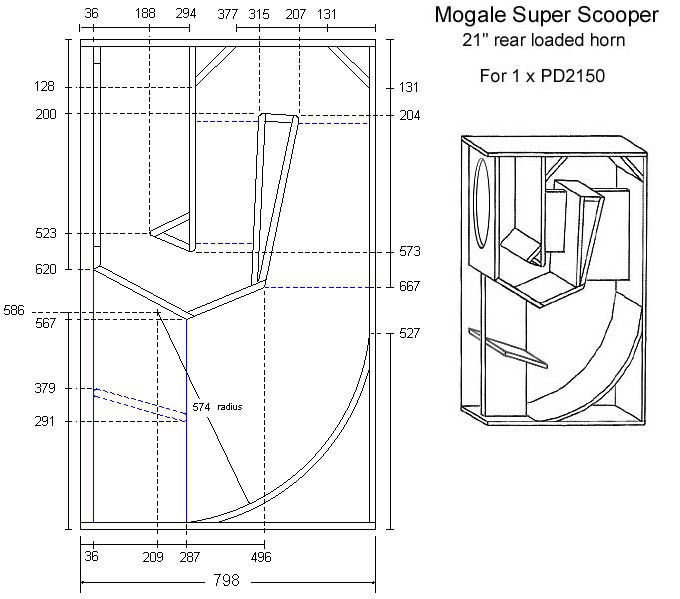
\includegraphics[scale=0.5]{21MogaleSuperScooper.jpg}
    \caption{Vista de perfil del 21" \ Mogale Super Scooper}
    \label{fig:logoETSII}
\end{figure}

En la inmensa mayoría de casos el tamaño original de la imagen no se adapta correctamente a las dimensiones de la página, por lo que es necesario redimensionar la imagen mediante el argumento \texttt{scale} de \textbackslash\texttt{includegraphics}. 

Al igual que para las tablas, existen distintas alternativas en cuanto a su posicionamiento (que, se recuerda, pueden consultarse en \url{https://www.overleaf.com/learn/latex/positioning_images_and_tables}), el título se indica mediante el comando \textbackslash\texttt{caption} y la referencia mediante el comando \textbackslash\texttt{label}. 

Existen, además, diversas opciones en lo relativo al manejo de imágenes que no se detallan en este documento, pero que pueden consultarse en \url{https://es.overleaf.com/learn/latex/Inserting_Images} 

%%%%%%%%%%%%%%%%%%%%%%%%%%%%%%%%%%%%%%%%%%%%%%%%%%


%%%%%%%%%%%%%%%%% - ECUACIONES - %%%%%%%%%%%%%%%%%

\newpage
\section{ECUACIONES} \label{sec:ecuaciones}

Una de las mayores ventajas de \LaTeX \ es lo fácil y rápido que resulta incorporar ecuaciones en el documento. Las ecuaciones se definen en el entorno \texttt{equation}, mediante el cual la identidad de Euler, por ejemplo, quedaría como:

\begin{equation}
    e^{i\pi} + 1 = 0
    \label{eq:euler}
\end{equation}

o la serie de Leibniz:

\begin{equation}
    \sum_{n=0}^\infty \frac{(-1)^n}{2n+1} = \frac{\pi}{4}
    \label{eq:leibniz}
\end{equation}

Como se puede ver, las ecuaciones se numeran de forma automática con respecto al capítulo en el que se encuentran (para no numerar una ecuación basta con definir el entorno como \textbackslash\texttt{begin\{equation*\}}), número al que se puede hacer referencia definiendo el comando \textbackslash\texttt{label}.

En este apartado se utilizan algunos de los símbolos matemáticos básicos, para más información sobre los distintos comandos que corresponden a diversos símbolos puede consultarse \url{https://www.caam.rice.edu/~heinken/latex/symbols.pdf}.


\subsection{Ecuaciones en el texto}

También existe la posibilidad de introducir expresiones matemáticas en una línea de texto encerrando la expresión entre dos símbolos \$, mediante lo cual se puede hacer referencia al número complejo $i$, que puede definirse como $\sqrt{-1}=i$, sin necesidad de interrumpir la oración.


\subsection{Entorno \textbackslash\texttt{split}}

En el caso de que una ecuación sea demasiado larga como para caber en una única línea puede usarse el entorno \texttt{split}, utilizado para el desarrollo de la serie de Taylor de $\sin{x}$ que aparece a continuación:

\begin{equation}
\begin{split}
    \sin{x} = \ & x - \frac{x^3}{3!} + \frac{x^5}{5!} - \frac{x^7}{7!} + \frac{x^9}{9!} - \frac{x^{11}}{11!} + \frac{x^13}{13!} + \dots \\ & + (-1)^n \frac{x^{2n+1}}{(2n+1)!} + \dots \qquad , \forall x \in \mathbb{R}
    \label{eq:taylor}
\end{split}
\end{equation}

La disposición de la ecuación no se hace automáticamente, por lo que es necesario indicar en qué lugar quedan verticalmente alineadas las distintas líneas (esto se realiza mediante el símbolo \& que en este caso va colocado después del $=$ en la primera línea y antes del primer $+$ de la segunda línea) y en qué momento se salta a la línea (que se indica mediante el comando \textbackslash\textbackslash).


\subsection{La herramienta Mathpix}

Mathpix es una aplicación que permite traducir a lenguaje \LaTeX \ cualquier ecuación, ya se encuentre en un archivo PDF o escrita a mano en un folio de papel. Aunque el proceso de plasmar ecuaciones en un documento \LaTeX \ ya es sencillo y rápido, esta herramienta lo vuelve casi instantáneo. La aplicación puede descargarse desde la página web de Mathpix: \url{https://mathpix.com/}.

%%%%%%%%%%%%%%%%%%%%%%%%%%%%%%%%%%%%%%%%%%%%%%%%%%

%%%%%%%%%%%%%%%% - BIBLIOGRAFÍA - %%%%%%%%%%%%%%%%

\newpage

El formato elegido para la bibliografía es APA (el recomendable para informes de TFG/TFM), tanto para las referencias a lo largo del documento como para el apartado de bibliografía. El conjunto de operaciones realizadas para establecer el formato de la bibliografía se puede consultar en el preámbulo del documento (en el que se describen algunos de sus parámetros básicos como el contenido de las referencias, el número de autores por cita, etc.).

Citar una referencia es sencillo, basta con utilizar el comando \textbackslash\texttt{cite} seguido del nombre de la referencia correspondiente (el nombre utilizado en el archivo \textit{.bib}, que es esencial cargar en el directorio de trabajo y cuyas principales características pueden consultarse en \url{https://en.wikipedia.org/wiki/BibTeX}), por ejemplo:

\begin{itemize}
    \item \textit{The Art of Electronics} constituye un fantástico manual (plagado de ejemplos prácticos y explicaciones tangibles) para aprender electrónica, siendo su tercera edición la versión más completa (\cite{horowitz2015}).
    \item \textit{The Loudspeaker Design Cookbook} (\cite{dickson2007}) es probablemente la guía más completa en cuanto a acústica aplicada al diseño de sistemas de sonido, abarcando desde conceptos teóricos de electroacústica hasta planos para la construcción de sistemas de sonido caseros.
    \item \textit{Les fous du son} (\cite{dewilde2016}) es un relato cuidadosamente escrito y documentado sobre la historia de los sintetizadores desde Edison hasta nuestros días, pasando por los inventos más inverosímiles como las Ondas Martenot o el Trautonium.
    \item En su artículo de 2003 (\cite{wang2003}), el co-fundador de Shazam describe el funcionamiento de su algoritmo de búsqueda para archivos de audio.
\end{itemize}

% Se genera la bibliografía mediante el comando \printbibliography (en ella aparecen únicamente las referencias citadas a lo largo del documento):
\appto{\bibsetup}{\sloppy}
\printbibliography[heading=bibintoc, title=BIBLIOGRAFÍA] % el argumento "title" puede modificarse indicando el título que convenga (bibliografía, referencias, etc.).

%%%%%%%%%%%%%%%%%%%%%%%%%%%%%%%%%%%%%%%%%%%%%%%%%%


%%%%%%%%%%%%%%%%%%% - ANEXOS - %%%%%%%%%%%%%%%%%%%

\newpage

\section*{ANEXOS} \label{sec:anexos} % Se añade un asterisco a \section para que el título no esté numerado.
\addcontentsline{toc}{section}{ANEXOS} % Al utilizar \section* se ha de añadir manualmente el apartado al índice (Table Of Contents, TOC).
\markright{ANEXOS} % Al utilizar \section* se ha de añadir manualmente el título del apartado al encabezado.

\renewcommand{\thesubsection}{\Alph{subsection}} % Se numeran los anexos con letras del alphabeto en lugar de números.
% Se indica que las tablas, figuras y códigos se numeran con el código del anexo (A, B, C, ...) seguido del número de tabla, figura o código dentro del anexo (tabla A.2, figura C.1, etc.)
\renewcommand{\thetable}{\Alph{subsection}.\arabic{table}}
\renewcommand{\thefigure}{\Alph{subsection}.\arabic{figure}}
\renewcommand{\thecode}{\Alph{subsection}.\arabic{code}}

% ---------------- Primer anexo ---------------- %
\subsection{Primer anexo} \label{sec:anexo1}

Contenido del primer anexo (texto, tablas, figuras, códigos, etc.)

% ---------------- Segundo anexo --------------- %
\newpage
\subsection{Segundo anexo} \label{sec:anexo2}

%%%%%%%%%%%%%%%%%%%%%%%%%%%%%%%%%%%%%%%%%%%%%%%%%%


%%%%%%%%%%%%%% - ÍNDICE DE TABLAS - %%%%%%%%%%%%%%

\newpage

\renewcommand{\listtablename}{ÍNDICE DE TABLAS} % Se define el nombre del índice de tablas.
\listoftables % Se genera automáticamente el índice con las distintas tablas del documento (entorno \table o \longtable).
\addcontentsline{toc}{section}{ÍNDICE DE TABLAS} % Se añade manualmente el apartado al índice (Table Of Contents, TOC).

%%%%%%%%%%%%%%%%%%%%%%%%%%%%%%%%%%%%%%%%%%%%%%%%%%


%%%%%%%%%%%%% - ÍNDICE DE FIGURAS - %%%%%%%%%%%%%%

\newpage

\renewcommand{\listfigurename}{ÍNDICE DE FIGURAS} % Se define el nombre del índice de figuras.
\listoffigures % Se genera automáticamente el índice con las distintas figuras del documento (entorno \figure).
\addcontentsline{toc}{section}{ÍNDICE DE FIGURAS} % Se añade manualmente el apartado al índice (Table Of Contents, TOC).

%%%%%%%%%%%%%%%%%%%%%%%%%%%%%%%%%%%%%%%%%%%%%%%%%%


%%%%%%%%%%%%%% - ÍNDICE DE CÓDIGOS - %%%%%%%%%%%%%

\newpage

\listofcodes % Se genera automáticamente el índice con los distintos códigos del documento (entorno \code).
\addcontentsline{toc}{section}{ÍNDICE DE CÓDIGOS} % Se añade manualmente el apartado al índice (Table Of Contents, TOC).

\afterpage{\blankpage} % Se añade una página en blanco después del índice de códigos.

%%%%%%%%%%%%%%%%%%%%%%%%%%%%%%%%%%%%%%%%%%%%%%%%%%



%%%%%%%%%%%%%%%%%%%%%%%%%%%%%%%%%%%%%%%%%%%%%%%%%%


%%%%%%%%%%%%%% - FIN DEL DOCUMENTO - %%%%%%%%%%%%%

\end{document}

%%%%%%%%%%%%%%%%%%%%%%%%%%%%%%%%%%%%%%%%%%%%%%%%%%
